% ==============================================================
% 2 - Preliminaries
% ==============================================================
\chapter{Preliminaries} \label{sec: Preliminaries}

\lipsum[1-3]

\begin{figure}[htb!] \centering
    \caption{A dog, the inverse of a god.}

    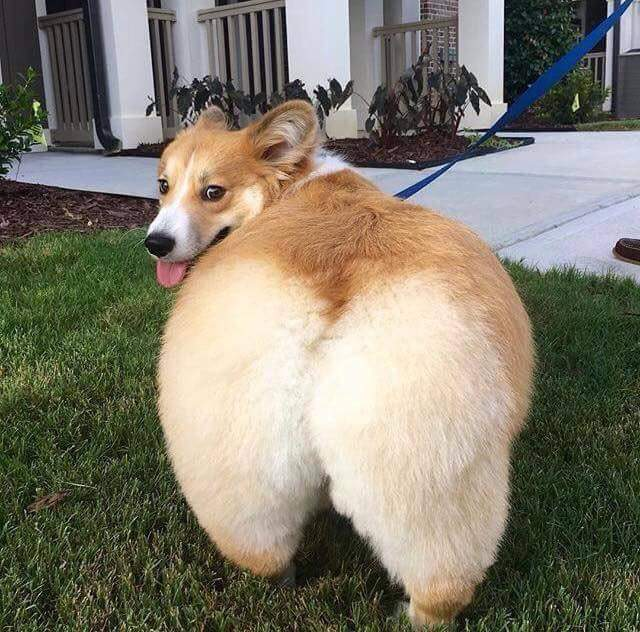
\includegraphics[width=0.6\textwidth]{imgs/dog.jpg}

    Source: Prepared by the author.
    \label{fig: Corgi}
\end{figure}

\lipsum[4-5]
\begin{align*}
    \dot{x}(t) &= A(t) x(t) + B(t) u(t) \\
          y(t) &= C(t) x(t) + D(t) u(t)
\end{align*}

\lipsum[6-8]